\documentclass[journal]{IEEEtran}
\usepackage{amsmath,amssymb,amsfonts,amsthm,mathtools,bm,mathrsfs}
\usepackage{graphicx}
\usepackage{booktabs,array}
\usepackage{algorithm}
\usepackage{algpseudocode}
\usepackage{tikz}
\usetikzlibrary{arrows.meta,positioning,fit,calc}
\usepackage{cite}
\usepackage{url}
\usepackage{microtype}

\newtheorem{theorem}{Theorem}
\newtheorem{proposition}{Proposition}
\newtheorem{assumption}{Assumption}
\newtheorem{remark}{Remark}
\newtheorem{corollary}{Corollary}
\newcommand{\norm}[1]{\left\lVert #1\right\rVert}
\newcommand{\abs}[1]{\left\lvert #1\right\rvert}
\newcommand{\T}{\mathsf T}
\newcommand{\1}{\bm 1}

\title{Measurement-Decoupled Attention--Koopman--T--S Fuzzy Monitoring via Structured Basis-Perturbation Residual Learning}
\author{Anonymous Authors}

\begin{document}
\maketitle

\begin{abstract}
This paper addresses normal-data-only monitoring of closed-loop nonlinear
systems when physical fault channels, directions, temporal profiles, and
labeled fault samples are unavailable. First, a strictly causal attention
encoder is coupled with a Takagi--Sugeno (T--S) fuzzy Koopman model to construct
a measurement-decoupled normal reference. A start-indexed residual then gives
the same mathematical object for free-rollout training, short-horizon
monitoring, and long-reference monitoring. Second, the complete fuzzy Koopman
Jacobian is decomposed into the interpolated local dynamics and the variation
of normalized rule weights. This yields an implementable infinity-norm
propagation bound and a reliable reference horizon without eigenvalue,
singular-value, inverse-matrix, or higher-order derivative operations during
training. Third, model-internal basis perturbations are applied separately to
input, measurement, and lifted coordinates. Ordinary forward rollouts produce
finite-horizon residual responses used to jointly reduce normal propagation,
increase perturbation sensitivity, and separate response patterns. Online
scores are standardized by fuzzy operating region, controller command,
command variation, and reference age, and their thresholds are calibrated
using held-out normal blocks. Sufficient residual-space conditions are derived
for detection and unique group separation. When the conditions for a unique
decision fail, the method returns a set of compatible perturbation groups
rather than an unsupported physical fault label.
\end{abstract}

\begin{IEEEkeywords}
Attention, fault detection, Koopman operator, normal-data-only learning,
structured perturbation, Takagi--Sugeno fuzzy systems.
\end{IEEEkeywords}

\section{Introduction}
\IEEEPARstart{N}{onlinear} closed-loop systems frequently operate across
multiple regimes while providing few representative fault records. Learning
normal input--output behavior is therefore attractive for monitoring, but it
creates a structural difficulty: the same measurement may be used both to
form a residual and to update the state and model against which that residual
is evaluated. When an abnormal measurement updates an encoder, an attention
context, or a fuzzy scheduling variable, the reference may move with the
abnormal trajectory and reduce the discrepancy intended for detection.

Koopman learning seeks lifted coordinates in which nonlinear dynamics admit a
finite-dimensional approximation \cite{brunton2016,lusch2018}. T--S fuzzy
models interpolate local linear descriptions through normalized firing
strengths \cite{takagi1985,tanaka2001,lam2018}. Their combination has already
been investigated in modeling and predictive control \cite{hu2026}; the
combination itself is consequently not claimed as a contribution here. The
T--S structure is instead made operational in three places: the normal
reference, the finite-horizon error propagation, and the
operating-condition-dependent monitoring rule. Attention is retained to
represent long input--output histories, but its output is prevented from
feeding new measurements into the normal reference after initialization.

Classical fuzzy fault-detection methods commonly introduce explicit fault or
unknown-input channels and then design observers or filters by Lyapunov and
linear-matrix-inequality techniques
\cite{nguang2007,yang2011,thumati2014,zhao2020,ran2022}. Koopman-based fault
diagnosis has also used learned residual and parity relations
\cite{bakhtiaridoust2023,irani2024}. Those formulations are appropriate when a
physical fault model or representative fault data are available. In the
setting considered here, training data are normal, and the physical fault
location, direction, and time profile are unknown. A physical minimum fault
gain cannot therefore be identified. The available structure is limited to
the known input and measurement coordinates and to the coordinates of the
learned lifted model.

This information boundary creates one connected design problem. Removing new
measurements from the reference prevents adaptation to abnormal observations,
but also exposes normal free-rollout drift. Reducing only that drift is
insufficient because a less sensitive model may reduce abnormal residuals as
well. Finally, an unknown physical fault direction precludes a justified
low-dimensional fault-sensitive projection. The method must instead control
normal propagation, retain the joint residual, and learn separable responses
only for explicitly defined model-coordinate perturbation groups.

The principal contributions are as follows.
\begin{enumerate}
\item A measurement-decoupled attention--Koopman--T--S reference and a
start-indexed residual are constructed. They unify free-rollout training,
short-horizon monitoring, and long-reference monitoring, and yield an exact
nonlinear residual recursion together with a delay-confirmed anchor rule.

\item The complete T--S fuzzy Koopman Jacobian is decomposed to expose the
effects of local dynamics, rule overlap, local-model disparity, and scheduling
sensitivity. An infinity-norm bound, enforced by elementwise parameterization,
gives a finite-horizon normal residual bound and a reliable reference horizon
without costly or poorly differentiable matrix operations.

\item Perturbation rollouts applied to the input, measurements, and lifted
coordinates are integrated with normal-propagation learning. The resulting
input-conditioned statistic admits sufficient residual-space detection and
group-separation conditions and returns a set-valued decision when a unique
group is not supported.
\end{enumerate}

The remainder of the paper is organized as follows. Section~II specifies the
information boundary and formulates three aligned subproblems. Section~III
develops the model, reference, propagation analysis, and structured response
learning. Section~IV gives the input-conditioned detection and set-valued
isolation method. Section~V concludes the paper.

Throughout the paper, the superscripts $\mathfrak n$ and $\mathfrak f$
identify quantities associated with normal and faulty operation,
respectively. The subscript $0$ is reserved for an initial value.

\section{Preliminaries and Problem Formulation}
\subsection{Information Boundary and Controlled-Process Description}
Let $\bm u_k\in\mathbb R^{m_u}$ be the controller command recorded online and
let $\bm u_k^{\rm a}\in\mathbb R^{m_u}$ be the actuator output actually
applied to the controlled process; $\bm u_k^{\rm a}$ need not be measured.
The fault-inclusive controlled process is described by
\begin{equation}
\begin{aligned}
\bm u_k^{\rm a}&=\bm u_k+\bm f_k^{\rm a},\\
\bm x_{k+1}&=\mathcal X^{\mathfrak n}
(\bm x_k,\bm u_k^{\rm a})
+\bm f_k^{\rm p}+\bm\varepsilon_k^x,\\
\bm y_k&=\mathcal Y^{\mathfrak n}
(\bm x_k,\bm u_k^{\rm a})
+\bm f_k^{\rm s}+\bm\varepsilon_k^y,
\end{aligned}
\label{eq:controlled_process}
\end{equation}
where $\bm x_k\in\mathbb R^{m_x}$ and
$\bm y_k\in\mathbb R^{m_y}$ denote the physical state and measured output,
respectively. The additive vectors
$\bm f_k^{\rm a}\in\mathbb R^{m_u}$,
$\bm f_k^{\rm p}\in\mathbb R^{m_x}$, and
$\bm f_k^{\rm s}\in\mathbb R^{m_y}$ represent possible actuator-side,
process-side, and measurement-side deviations. The normal-operation mappings
$\mathcal X^{\mathfrak n}:\mathbb R^{m_x}\times\mathbb R^{m_u}
\rightarrow\mathbb R^{m_x}$ and
$\mathcal Y^{\mathfrak n}:\mathbb R^{m_x}\times\mathbb R^{m_u}
\rightarrow\mathbb R^{m_y}$ are unknown. The dimensions of the fault vectors
specify only their possible physical locations; they do not provide known
fault directions to the learning algorithm.

Only $\bm u_k$ and $\bm y_k$ are assumed available online for fault diagnosis.
Using the recorded controller command in the normal model answers the
conditional question: how should the controlled process evolve under this
command if its actuator and dynamics follow the normal-operation model? A
command modified by a feedback controller after an abnormal measurement
remains a known conditioning variable, whereas an unmeasured difference
between $\bm u_k^{\rm a}$ and $\bm u_k$ remains an inconsistency to be
detected.

Only normal trajectories are used for model training and threshold
calibration. No physical fault matrix, fault direction, fault derivative,
fault time model, or labeled fault trajectory is used. Model parameters and
calibration quantities are frozen during testing. Define the strictly past
history
\begin{equation}
\mathcal H_k^-=
\left\{\bm u_{k-\ell_h:k-1},\,
\bm y_{k-\ell_h:k-1}\right\},
\label{eq:history}
\end{equation}
where the current output $\bm y_k$ is excluded.

\subsection{Finite-History Lifted Representation}
For the normal-operation dynamics, Koopman evolution acts on an observable by
composition with the state transition \cite{brunton2016}. A finite vector of
observables $\bm\psi:\mathbb R^{m_x}\rightarrow\mathbb R^{m_z}$
would satisfy the ideal composition relation
\begin{equation}
\bm\psi\!\left(\mathcal X^{\mathfrak n}(\bm x_k,\bm u_k)\right)
=\bm\psi(\bm x_{k+1}).
\label{eq:koopman}
\end{equation}
The paper does not assume that a finite invariant subspace exists or that the
learned lifted coordinates contain the physical state. Instead, a
finite-history encoder estimates a predictive coordinate
$\bm z_k^{\rm enc}\in\mathbb R^{m_z}$ from \eqref{eq:history}, and a T--S
interpolation
of local lifted linear models approximates \eqref{eq:koopman} on the normal
operating domain. Approximation and finite-history errors are retained in the
residual propagation derived in Section~III.

\subsection{Problem Formulation}
Under the preceding information boundary, this paper addresses three
subproblems.
\begin{enumerate}
\item \emph{Reference construction:} construct a normal reference that uses
new measurements for residual evaluation but not for reference updates, while
using one residual definition in training and in both short- and long-horizon
testing.

\item \emph{Normal propagation:} quantify the finite-horizon drift of that
reference through the complete attention--Koopman--T--S mapping using
operations suitable for first-order network training, and make the realized
input and fuzzy operating region explicit.

\item \emph{Residual-space decision:} using normal data only, jointly reduce
normal residual propagation and increase separability of reproducible
model-coordinate perturbation responses; then construct an input-conditioned
detection statistic and return a unique group only when the residual response
supports it.
\end{enumerate}

\section{Proposed Method}
\subsection{Attention--Koopman--T--S Normal Model}
Each element of \eqref{eq:history} is embedded as a token $\bm h_j$. For
attention head $q\in\{1,\ldots,m_{\rm hd}\}$, the strictly causal coefficient
assigned at sample $k$ to a past token $j$ is
\begin{equation}
\varpi_{k,j}^{(q)}
=\frac{\exp\!\left(
(\bm W_Q^{(q)}\bm h_{k-1})^\T
(\bm W_K^{(q)}\bm h_j)/\sqrt{m_{\rm a}}\right)}
{\displaystyle\sum_{\ell=k-\ell_h}^{k-1}
\exp\!\left(
(\bm W_Q^{(q)}\bm h_{k-1})^\T
(\bm W_K^{(q)}\bm h_\ell)/\sqrt{m_{\rm a}}\right)}.
\label{eq:attention}
\end{equation}
The head outputs are concatenated to form
\begin{equation}
\begin{aligned}
\bm\chi_k&=\bm W_O
\left[
\sum_{j=k-\ell_h}^{k-1}\varpi_{k,j}^{(q)}
\bm W_V^{(q)}\bm h_j
\right]_{q=1}^{m_{\rm hd}},
\\
\bm z_k^{\rm enc}&=\mathcal H_\Theta(\mathcal H_k^-).
\end{aligned}
\label{eq:encoder}
\end{equation}
The encoder in \eqref{eq:encoder} includes the token embeddings and the
multihead attention operation. Equation~\eqref{eq:attention} makes the causal
information path explicit; attention itself is not treated as a separate
contribution.

The scheduling vector is
\begin{equation}
\bm\rho_k=\bm W_z\bm z_k+\bm W_\chi\bm\chi_k+
\bm W_u\bm u_k.
\label{eq:schedule}
\end{equation}
Constant offsets are represented by an augmented constant coordinate. For
$i\in\{1,\ldots,m_r\}$, define
\begin{equation}
\begin{aligned}
\varphi_i(\bm\rho)
&=-\frac{1}{2}(\bm\rho-\bm c_i)^\T
\bm\Pi_i(\bm\rho-\bm c_i),\\
\omega_i(\bm\rho)
&=\frac{\exp(\varphi_i(\bm\rho))}
{\displaystyle\sum_{j=1}^{m_r}\exp(\varphi_j(\bm\rho))}.
\end{aligned}
\label{eq:fuzzy_weights}
\end{equation}
Thus, $\omega_i\geq0$ and $\sum_i\omega_i=1$. The diagonal metric is
parameterized by
\begin{equation}
\begin{aligned}
\bm\Pi_i&=\mathrm{Diag}\!\left[
\underline{\pi}\1+
(\overline{\pi}-\underline{\pi})
\operatorname{sigmoid}(\widetilde{\bm\pi}_i)\right],\\
\bm c_i&=\overline{\bm c}\odot\tanh(\widetilde{\bm c}_i).
\end{aligned}
\label{eq:metric_parameterization}
\end{equation}
where all operations inside the brackets are elementwise and
$0<\underline{\pi}<\overline{\pi}$. Cross-coordinate dependence is retained
through \eqref{eq:schedule}; consequently, the diagonal metric in the
scheduling space does not imply an axis-aligned partition of the original
history space.

The local and interpolated lifted models are
\begin{equation}
\begin{aligned}
\bm v_i(\bm z,\bm u)&=\bm A_i\bm z+\bm B_i\bm u,\\
\mathcal T_\Theta(\bm z,\bm u;\bm\chi)
&=\sum_{i=1}^{m_r}\omega_i(\bm\rho)\bm v_i(\bm z,\bm u),\\
\bm y^{\rm dec}&=\mathcal D_\Theta(\bm z,\bm u).
\end{aligned}
\label{eq:fuzzy_transition}
\end{equation}
The decoder $\mathcal D_\Theta$ is distinct from the physical output mapping
$\mathcal Y^{\mathfrak n}$. This distinction is necessary because the learned lifted state
need not contain the physical state.

The matrices that determine the propagation bound use elementwise hard
parameterizations, for example,
\begin{equation}
\begin{aligned}
[\bm A_i]_{pq}&=\frac{\kappa_A}{m_z}
\tanh([\widetilde{\bm A}_i]_{pq}),\\
[\bm B_i]_{pq}&=\frac{\kappa_B}{m_u}
\tanh([\widetilde{\bm B}_i]_{pq}),\\
[\bm W_z]_{pq}&=\frac{\kappa_W}{m_z}
\tanh([\widetilde{\bm W}_z]_{pq}).
\end{aligned}
\label{eq:hard_bounds}
\end{equation}
Hence $\norm{\bm A_i}_\infty\leq\kappa_A$,
$\norm{\bm B_i}_\infty\leq\kappa_B$, and
$\norm{\bm W_z}_\infty\leq\kappa_W$ by construction. No spectral projection
is required.

Training uses a normal training split and a free-rollout horizon
$\ell_{\rm tr}$. Starting from $\bm z_{s\mid s}^{\rm roll}=\bm z_s^{\rm enc}$,
the predicted output, rather than the new measurement, updates the rollout
history:
\begin{equation}
\begin{aligned}
\bm\chi_{t\mid s}^{\rm roll}
&=\mathcal H_\Theta^\chi(\mathcal H_{t\mid s}^{\rm roll}),\\
\bm z_{t+1\mid s}^{\rm roll}
&=\mathcal T_\Theta(\bm z_{t\mid s}^{\rm roll},\bm u_t;
\bm\chi_{t\mid s}^{\rm roll}),\\
\bm y_{t\mid s}^{\rm roll}
&=\mathcal D_\Theta(\bm z_{t\mid s}^{\rm roll},\bm u_t).
\end{aligned}
\label{eq:free_rollout}
\end{equation}
The normal prediction loss is
\begin{equation}
\begin{aligned}
\mathcal L_{\rm pred}
=\sum_s\sum_{\ell=1}^{\ell_{\rm tr}}\big(&
\lambda_z\norm{\bm z_{s+\ell}^{\rm enc}
-\bm z_{s+\ell\mid s}^{\rm roll}}_1\\
&+
\lambda_y\norm{\bm y_{s+\ell}
-\bm y_{s+\ell\mid s}^{\rm roll}}_1
\big).
\end{aligned}
\label{eq:prediction_loss}
\end{equation}
Free rollout, rather than one-step teacher forcing, matches the online
reference mechanism.

\begin{figure*}[t]
\centering
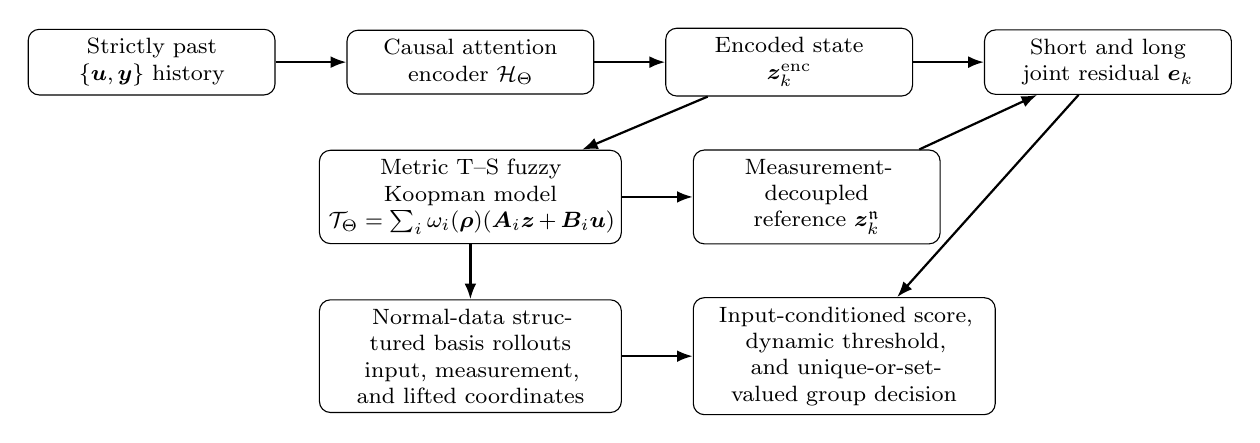
\begin{tikzpicture}[
node distance=7mm and 9mm,
box/.style={draw,rounded corners,align=center,minimum height=8mm,
text width=29mm,font=\footnotesize},
wide/.style={draw,rounded corners,align=center,minimum height=8mm,
text width=36mm,font=\footnotesize},
arr/.style={-{Latex[length=2mm]},thick}
]
\node[box] (hist) {Strictly past\\$\{\bm u,\bm y\}$ history};
\node[box,right=of hist] (enc) {Causal attention\\encoder $\mathcal H_\Theta$};
\node[box,right=of enc] (data) {Encoded state\\$\bm z_k^{\rm enc}$};
\node[wide,below=of enc] (fuzzy) {Metric T--S fuzzy Koopman model\\
$\mathcal T_\Theta=\sum_i\omega_i(\bm\rho)(\bm A_i\bm z+\bm B_i\bm u)$};
\node[box,right=of fuzzy] (ref) {Measurement-decoupled\\reference $\bm z_k^{\mathfrak n}$};
\node[box,right=of data] (res) {Short and long\\joint residual $\bm e_k$};
\node[wide,below=of fuzzy] (basis) {Normal-data structured basis rollouts\\
input, measurement, and lifted coordinates};
\node[wide,right=of basis] (dec) {Input-conditioned score, dynamic threshold,\\
and unique-or-set-valued group decision};
\draw[arr] (hist)--(enc);
\draw[arr] (enc)--(data);
\draw[arr] (data)--(res);
\draw[arr] (fuzzy)--(ref);
\draw[arr] (ref)--(res);
\draw[arr] (data)--(fuzzy);
\draw[arr] (basis)--(dec);
\draw[arr] (res)--(dec);
\draw[arr] (fuzzy)--(basis);
\end{tikzpicture}
\caption{Information paths of the proposed method. New measurements remain in
the data branch and residual, whereas the normal reference is propagated by
the frozen model, recorded command, and predicted outputs.}
\label{fig:architecture}
\end{figure*}

\subsection{Measurement-Decoupled Reference and Unified Residual}
For any start $s$, the rollout \eqref{eq:free_rollout} defines the lifted
residual
\begin{equation}
\bm e_{k\mid s}^z=\bm z_k^{\rm enc}-\bm z_{k\mid s}^{\rm roll},
\qquad k\geq s,
\label{eq:start_residual}
\end{equation}
and the output-consistency residual is
\begin{equation}
\bm e_k^y=\bm y_k-
\mathcal D_\Theta(\bm z_k^{\rm enc},\bm u_k).
\label{eq:output_residual}
\end{equation}
Equation~\eqref{eq:start_residual} is the same object used in
\eqref{eq:prediction_loss}. Online, $s=k-\ell_{\rm sh}$ gives a short rolling
residual. Let $s_k^{\mathfrak n}$ be the latest delay-confirmed normal anchor
and define
\begin{equation}
\bm z_k^{\mathfrak n}=\bm z_{k\mid s_k^{\mathfrak n}}^{\rm roll},\qquad
\ell_k^{\mathfrak n}=k-s_k^{\mathfrak n}.
\label{eq:normal_reference}
\end{equation}
Then $s=s_k^{\mathfrak n}$ gives the long-reference residual. The minimal
joint residual is
\begin{equation}
\bm e_k=
\begin{bmatrix}
(\bm e_k^y)^\T&
(\bm e_{k\mid k-\ell_{\rm sh}}^z)^\T&
(\bm e_{k\mid s_k^{\mathfrak n}}^z)^\T
\end{bmatrix}^{\T}.
\label{eq:joint_residual}
\end{equation}
Thus, training and testing do not introduce different lifted residuals; only
the rollout start changes.

An encoded state is not immediately accepted as a normal anchor. It is stored
as a candidate and committed after $\ell_{\rm cf}$ samples only if no warning
is issued for any window containing that candidate. During warning and alarm
intervals, the accepted anchor is frozen and \eqref{eq:free_rollout} continues
without measurement updates.

\begin{proposition}[Delayed anchor acceptance]
\label{prop:anchor}
Suppose every abnormal trajectory in a specified detectable class triggers a
warning within at most $\ell_{\rm det}$ samples after its onset. If
$\ell_{\rm cf}\geq\ell_{\rm det}$, no candidate generated at or after that
onset is committed before the warning.
\end{proposition}

\begin{proof}
A candidate requires $\ell_{\rm cf}$ consecutive warning-free samples before
commitment. Under the stated premise, a warning occurs no later than
$\ell_{\rm det}\leq\ell_{\rm cf}$ samples after onset, so a post-onset
candidate fails the acceptance condition.
\end{proof}

Proposition~\ref{prop:anchor} is conditional; faults that never change the
available input--output information cannot be covered. After an alarm clears,
the method waits at least $\ell_h$ samples, so that the encoder history no
longer contains the flagged interval, and then repeats delay confirmation.

Define the encoded-state innovation and the context mismatch as
\begin{equation}
\begin{aligned}
\bm\nu_k
&=\bm z_{k+1}^{\rm enc}
-\mathcal T_\Theta(\bm z_k^{\rm enc},\bm u_k;\bm\chi_k),\\
\bm\delta_{k\mid s}^{\chi}
&=\mathcal T_\Theta(\bm z_k^{\rm enc},\bm u_k;\bm\chi_k)
-\mathcal T_\Theta(\bm z_k^{\rm enc},\bm u_k;
\bm\chi_{k\mid s}^{\rm roll}).
\end{aligned}
\label{eq:innovation_context}
\end{equation}

\begin{theorem}[Exact start-indexed residual propagation]
\label{thm:exact}
Assume $\mathcal T_\Theta$ is continuously differentiable in $\bm z$ on the
line segment joining $\bm z_{k\mid s}^{\rm roll}$ and
$\bm z_k^{\rm enc}$. Then
\begin{equation}
\bm e_{k+1\mid s}^z
=\overline{\bm\Gamma}_{k\mid s}\bm e_{k\mid s}^z
+\bm\nu_k+\bm\delta_{k\mid s}^{\chi},
\label{eq:exact_recursion}
\end{equation}
where
\begin{equation}
\overline{\bm\Gamma}_{k\mid s}=
\int_0^1
\bm\Gamma_{z,k}\!\left(
\bm z_{k\mid s}^{\rm roll}
+\tau\bm e_{k\mid s}^z\right)\,\mathrm d\tau.
\label{eq:averaged_jacobian}
\end{equation}
Consequently,
\begin{equation}
\bm e_{k\mid s}^z=
\bm\Phi(k,s)\bm e_{s\mid s}^z+
\sum_{j=s}^{k-1}\bm\Phi(k,j+1)
(\bm\nu_j+\bm\delta_{j\mid s}^{\chi}),
\label{eq:finite_propagation}
\end{equation}
with $\bm\Phi(k,j)=
\overline{\bm\Gamma}_{k-1\mid s}\cdots
\overline{\bm\Gamma}_{j\mid s}$ and
$\bm\Phi(j,j)=\bm I$.
\end{theorem}

The proof follows by adding and subtracting the transition evaluated at the
encoded state and the rollout context, followed by the integral mean-value
identity; details are given in Appendix~A. The term $\bm\nu_k$ is the
one-step normal-model inconsistency, whereas
$\bm\delta_{k\mid s}^{\chi}$ retains the effect of finite attention memory.

\subsection{Fuzzy-Structure-Dependent Normal Propagation}
For compactness, define
$\bm v_{i,k}=\bm A_i\bm z_k+\bm B_i\bm u_k$ and
$\overline{\bm v}_k=\sum_i\omega_{i,k}\bm v_{i,k}$. From
\eqref{eq:fuzzy_weights},
\begin{equation}
\begin{aligned}
\bm\gamma_{i,k}^{\rho}
&:=\nabla_{\bm\rho}\varphi_{i,k}
=-\bm\Pi_i(\bm\rho_k-\bm c_i),\\
\overline{\bm\gamma}_k^{\rho}
&:=\sum_j\omega_{j,k}\bm\gamma_{j,k}^{\rho},\\
\nabla_{\bm\rho}\omega_{i,k}
&=\omega_{i,k}
(\bm\gamma_{i,k}^{\rho}-\overline{\bm\gamma}_k^{\rho}).
\end{aligned}
\label{eq:weight_gradient}
\end{equation}

\begin{theorem}[Complete fuzzy lifted-state Jacobian]
\label{thm:jacobian}
For fixed $\bm u_k$ and $\bm\chi_k$, the Jacobian of
\eqref{eq:fuzzy_transition} with respect to $\bm z$ is
\begin{equation}
\begin{aligned}
\bm\Gamma_{z,k}
={}&\sum_{i=1}^{m_r}\omega_{i,k}\bm A_i\\
&+\sum_{i=1}^{m_r}\omega_{i,k}
(\bm v_{i,k}-\overline{\bm v}_k)
(\bm\gamma_{i,k}^{\rho}
-\overline{\bm\gamma}_k^{\rho})^\T\bm W_z .
\end{aligned}
\label{eq:complete_jacobian}
\end{equation}
Moreover,
\begin{equation}
\begin{aligned}
\norm{\bm\Gamma_{z,k}}_\infty\leq\kappa_k:={}&
\sum_i\omega_{i,k}\norm{\bm A_i}_\infty\\
&+\norm{\bm W_z}_\infty
\sum_i\omega_{i,k}
\norm{\bm v_{i,k}-\overline{\bm v}_k}_\infty\\
&\hspace{14mm}\times
\norm{\bm\gamma_{i,k}^{\rho}
-\overline{\bm\gamma}_k^{\rho}}_1 .
\end{aligned}
\label{eq:jacobian_bound}
\end{equation}
\end{theorem}

Equation~\eqref{eq:complete_jacobian} separates the interpolated local dynamics
from the change in normalized firing strengths. The second term becomes large
only when rules overlap, their local next-state values differ, and the
scheduling vector is sensitive in a direction that changes their relative
weights. This is the specific role of the fuzzy structure in the reference
analysis. The proof and the induced-norm bound are given in Appendix~B.

\begin{assumption}[Normal residual forcing]
\label{ass:normal}
On a prescribed normal operating domain, known nonnegative values
$\overline{\varepsilon}_k$ satisfy
\begin{equation}
\norm{\bm\nu_k+\bm\delta_{k\mid s}^{\chi}}_\infty
\leq\overline{\varepsilon}_k
\label{eq:forcing_bound}
\end{equation}
on the calibrated normal event.
\end{assumption}

The values in Assumption~\ref{ass:normal} are not claimed as deterministic
global bounds obtained from finite data. The structural part of the bound
comes from \eqref{eq:hard_bounds}--\eqref{eq:jacobian_bound}; the unresolved
normal remainder is calibrated on held-out normal blocks in Section~IV.

\begin{corollary}[Finite-horizon normal residual bound]
\label{cor:bound}
If $\beta_{s\mid s}\geq\norm{\bm e_{s\mid s}^z}_\infty$ and
\begin{equation}
\beta_{k+1\mid s}=\kappa_k\beta_{k\mid s}
+\overline{\varepsilon}_k,
\label{eq:beta_recursion}
\end{equation}
then $\norm{\bm e_{k\mid s}^z}_\infty\leq\beta_{k\mid s}$ while the trajectory
remains in the prescribed normal domain. For an allowed reference tolerance
$\overline{\beta}$, a reliable horizon is
\begin{equation}
\ell_{\rm ref}(s)=
\max\left\{\ell:\beta_{s+j\mid s}\leq\overline{\beta},
\ 1\leq j\leq\ell\right\}.
\label{eq:reliable_horizon}
\end{equation}
\end{corollary}

All quantities in \eqref{eq:jacobian_bound} use matrix products, elementwise
absolute values, and row or column sums. The empirical training counterpart
of \eqref{eq:beta_recursion},
\begin{equation}
\mathcal L_{\rm nr}=
\sum_s\sum_{\ell=1}^{\ell_{\rm tr}}
\beta_{s+\ell\mid s}^{\rm emp},
\label{eq:normal_propagation_loss}
\end{equation}
is used only as a normal-reference propagation regularizer. It is not by
itself a claim of improved physical fault sensitivity.

\subsection{Structured Basis-Perturbation Residual Learning}
Reducing \eqref{eq:normal_propagation_loss} controls only the normal side of
residual separation. To create a diagnostic training signal without physical
fault data, define the model-coordinate group set
\begin{equation}
\mathbb G_{\rm b}=\{\mathrm u,\mathrm y,\mathrm z\},
\label{eq:group_set}
\end{equation}
representing input-, measurement-, and lifted-coordinate perturbations. These
groups specify where a perturbation is inserted in the learned architecture;
they are not physical actuator, sensor, or process labels.

At a sampled start $s$, select one standard basis vector and signed amplitude
$\alpha$. The input branch replaces $\bm u_s$ by
$\bm u_s+\alpha\bm q_j^u$ in the model rollout. The measurement branch
replaces $\bm y_s$ by $\bm y_s+\alpha\bm q_j^y$ in the current output residual
and in subsequent causal histories. The lifted branch uses
\begin{equation}
\bm z_{s+1}^{(\mathrm z,j,\alpha)}
=\mathcal T_\Theta(\bm z_s^{\rm enc},\bm u_s;\bm\chi_s)
+\alpha\bm q_j^z.
\label{eq:lifted_perturbation}
\end{equation}
Thereafter, every branch follows the same frozen model and reference logic as
the unperturbed normal branch. Denote its joint residual at sample $t$ by
$\bm e_t^{\mathfrak n}$.

For horizon $\ell_{\rm b}$, stack the branch residuals and subtract the
normal residual stack:
\begin{equation}
\Delta\bm e_{s,\ell_{\rm b}}^{g,j,\alpha}
=
\begin{bmatrix}
(\bm e_s^{g,j,\alpha}-\bm e_s^{\mathfrak n})^\T&
\cdots&
(\bm e_{s+\ell_{\rm b}-1}^{g,j,\alpha}
-\bm e_{s+\ell_{\rm b}-1}^{\mathfrak n})^\T
\end{bmatrix}^{\T}.
\label{eq:response_increment}
\end{equation}
Define the scaled response and its unit-$\ell_1$ pattern by
\begin{equation}
\eta_{g,j,\alpha}^{\rm rsp}=
\frac{\norm{\Delta\bm e_{s,\ell_{\rm b}}^{g,j,\alpha}}_1}
{\abs{\alpha}+\epsilon_{\rm reg}},
\qquad
\bm p_{g,j,\alpha}=
\frac{\abs{\Delta\bm e_{s,\ell_{\rm b}}^{g,j,\alpha}}}
{\norm{\Delta\bm e_{s,\ell_{\rm b}}^{g,j,\alpha}}_1+\epsilon_{\rm reg}},
\label{eq:response_pattern}
\end{equation}
where the absolute value in the numerator is elementwise and
$\epsilon_{\rm reg}>0$ is numerical regularization.

The sensitivity and intergroup separation losses are
\begin{equation}
\begin{aligned}
\mathcal L_{\rm sen}
&=\sum_{g,j,\alpha}
\left[\underline{\eta}_g-\eta_{g,j,\alpha}^{\rm rsp}\right]_+^2,\\
\mathcal L_{\rm iso}
&=\sum_{g\ne\bar g}
\left[
\eta_{\rm iso}
-\norm{\bm p_{g,j,\alpha}
-\bm p_{\bar g,\bar j,\bar\alpha}}_1
\right]_+^2.
\end{aligned}
\label{eq:response_losses}
\end{equation}
The complete objective is
\begin{equation}
\mathcal L=
\mathcal L_{\rm pred}
+\lambda_{\rm nr}\mathcal L_{\rm nr}
+\lambda_{\rm sen}\mathcal L_{\rm sen}
+\lambda_{\rm iso}\mathcal L_{\rm iso}
+\lambda_{\rm bal}\mathcal L_{\rm bal},
\label{eq:complete_loss}
\end{equation}
where $\mathcal L_{\rm bal}$ penalizes only rule occupancies below a prescribed
minimum; it does not force uniform rule usage. Each mini-batch samples one
coordinate from each group, so the additional computation consists of three
ordinary forward rollouts and first-order backpropagation. No Hessian,
eigendecomposition, singular-value decomposition, matrix inverse, or online
optimization is introduced.

\section{Input-Conditioned Detection and Set-Valued Isolation}
\subsection{Input-Conditioned Residual Standardization}
The normal distribution of \eqref{eq:joint_residual} depends on the realized
command, command variation, fuzzy operating region, and reference age. Define
\begin{equation}
\bm\upsilon_k=\bm u_k-\bm u_{k-1},\qquad
\bm\zeta_k=
\begin{bmatrix}
(\bm\omega_k^{\mathfrak n})^\T&
\bm u_k^\T&
\bm\upsilon_k^\T&
\ell_k^{\mathfrak n}
\end{bmatrix}^{\T},
\label{eq:descriptor}
\end{equation}
where $\bm\omega_k^{\mathfrak n}$ contains the firing strengths evaluated
along $\bm z_k^{\mathfrak n}$ and its predicted context. For each fuzzy rule,
normal training
blocks provide a local mean $\bm\mu_i(\bm\zeta_k)$ and positive elementwise
scale $\bm\sigma_i(\bm\zeta_k)$. Their mixture moments are
\begin{equation}
\begin{aligned}
\bm\mu_k&=\sum_i\omega_{i,k}^{\mathfrak n}\bm\mu_i,\\
\bm\sigma_k^{\odot2}
&=\sum_i\omega_{i,k}^{\mathfrak n}
\left[
\bm\sigma_i^{\odot2}
+(\bm\mu_i-\bm\mu_k)^{\odot2}
\right]+\epsilon_\sigma\1 .
\end{aligned}
\label{eq:mixture_moments}
\end{equation}
The between-rule term in \eqref{eq:mixture_moments} prevents uncertainty at a
rule boundary from being underestimated. Standardization is elementwise:
\begin{equation}
\widetilde{\bm e}_k=
(\bm e_k-\bm\mu_k)\oslash\bm\sigma_k.
\label{eq:standardized_residual}
\end{equation}

For each window length $\ell$ in a predeclared finite list, define
\begin{equation}
\varsigma_{k,\ell}=
\sum_{j=k-\ell+1}^{k}\norm{\widetilde{\bm e}_j}_1.
\label{eq:window_score}
\end{equation}
A held-out normal calibration split is partitioned by predeclared fuzzy
operating cells and reference-age intervals. Within each cell, nonoverlapping
blocks calibrate the upper quantile
$\tau_{\rm cal}(\bm\zeta_k,\ell)$. The propagated component from
\eqref{eq:beta_recursion}, after the same elementwise scaling, is denoted by
$\tau_{\rm prop}(\beta_{k\mid s_k^{\mathfrak n}},\ell)$. The online threshold
is
\begin{equation}
\tau_{k,\ell}=
\tau_{\rm cal}(\bm\zeta_k,\ell)
+\tau_{\rm prop}(\beta_{k\mid s_k^{\mathfrak n}},\ell).
\label{eq:dynamic_threshold}
\end{equation}
Thus, the raw normal region changes with the input, input variation, fuzzy
region, and reference age. The calibration term controls the unresolved
random remainder, whereas the propagation term records reference drift.

The multiscale statistic is
\begin{equation}
\varsigma_k^{\max}=
\max_{\ell\in\{\ell_1,\ldots,\ell_{\max}\}}
\frac{\varsigma_{k,\ell}}{\tau_{k,\ell}}.
\label{eq:multiscale}
\end{equation}
Its final decision level is calibrated directly on the maximum score, rather
than applying separate uncorrected tests to each window. A finite-sample
coverage interpretation requires exchangeable calibration and test blocks
within each declared cell; under serial dependence, the stated guarantee is
blockwise rather than samplewise \cite{vovk2005,xu2021}.

\subsection{Sufficient Detection Condition}
The following statement clarifies why normal propagation and structured
response learning must be used together.

\begin{proposition}[Residual-space detection]
\label{prop:detection}
For a selected window, suppose a normal standardized residual block
$\widetilde{\bm e}^{\,\mathfrak n}$ satisfies
$\norm{\widetilde{\bm e}^{\,\mathfrak n}}_1\leq\tau_{k,\ell}$ on the
calibrated normal event. Let the corresponding faulty residual block satisfy
$\widetilde{\bm e}^{\,\mathfrak f}
=\widetilde{\bm e}^{\,\mathfrak n}
+\Delta\widetilde{\bm e}^{\,\mathfrak f}$.
Suppose a structured perturbation produces the learned response
$\Delta\widetilde{\bm e}^{\,g,j,\alpha}$ and
$\norm{\Delta\widetilde{\bm e}^{\,\mathfrak f}
-\Delta\widetilde{\bm e}^{\,g,j,\alpha}}_1\leq\epsilon_g$. If
\begin{equation}
\norm{\Delta\widetilde{\bm e}^{\,g,j,\alpha}}_1
>2\tau_{k,\ell}+\epsilon_g,
\label{eq:detection_condition}
\end{equation}
then the corresponding residual block exceeds $\tau_{k,\ell}$ on that event.
\end{proposition}

Indeed, the reverse triangle inequality gives
$\norm{\widetilde{\bm e}^{\,\mathfrak f}}_1
>\tau_{k,\ell}$. If
\eqref{eq:response_losses} gives
$\norm{\Delta\widetilde{\bm e}^{\,g,j,\alpha}}_1
\geq\underline{\eta}_g\abs{\alpha}$, a sufficient amplitude condition is
\begin{equation}
\abs{\alpha}>
\frac{2\tau_{k,\ell}+\epsilon_g}{\underline{\eta}_g}.
\label{eq:amplitude_condition}
\end{equation}
Equation~\eqref{eq:amplitude_condition} is a residual-model conclusion, not a
physical minimum-fault claim. It shows the two controllable factors: reducing
normal propagation lowers $\tau_{k,\ell}$, and increasing the structured
response raises $\underline{\eta}_g$.

\subsection{Unique-or-Set-Valued Isolation}
After a detection, the observed residual increment is normalized as in
\eqref{eq:response_pattern}. For group $g$, let $\delta_g(k)$ be its smallest
$\ell_1$ distance to the response patterns stored from training rollouts. The
compatible set is
\begin{equation}
\mathbb G_k^{\rm cmp}=
\left\{g\in\mathbb G_{\rm b}:
\delta_g(k)\leq\tau_{\rm iso}\right\}.
\label{eq:candidate_set}
\end{equation}
A unique group is returned only when
$\mathbb G_k^{\rm cmp}$ contains one element and the distance to the
second-best group exceeds a calibrated ambiguity margin.

\begin{proposition}[Sufficient group separation]
\label{prop:isolation}
Suppose the observed normalized response lies within $\delta_{\rm obs}$ of a
stored pattern from its generating group. If every pattern from a different
group is at an $\ell_1$ distance greater than $2\delta_{\rm obs}$ from that
pattern, nearest-pattern classification returns the generating group.
\end{proposition}

The result follows from the triangle inequality. When its premise is not
satisfied, \eqref{eq:candidate_set} is the appropriate output. The labels
$\mathrm u$, $\mathrm y$, and $\mathrm z$ indicate compatibility with an
insertion location in the learned model. Without an independently verified
mapping, they must not be renamed as unique actuator, sensor, or process
faults.

\subsection{Offline and Online Algorithms}
Training, calibration, and testing use disjoint normal trajectory blocks.
Algorithm~\ref{alg:offline} summarizes the offline procedure.

\begin{algorithm}[H]
\caption{Normal-Data Offline Design}
\label{alg:offline}
\begin{algorithmic}[1]
\Require Disjoint normal training and calibration blocks
\State Train $\mathcal H_\Theta$, $\mathcal T_\Theta$, and
$\mathcal D_\Theta$ by free rollouts using \eqref{eq:prediction_loss}.
\State Apply \eqref{eq:metric_parameterization} and \eqref{eq:hard_bounds};
compute \eqref{eq:jacobian_bound} and \eqref{eq:normal_propagation_loss}.
\State Sample one coordinate from each group in \eqref{eq:group_set};
optimize \eqref{eq:complete_loss} with ordinary forward branches.
\State Freeze all model and fuzzy-rule parameters.
\State Estimate \eqref{eq:mixture_moments} and calibrate
\eqref{eq:dynamic_threshold} on held-out nonoverlapping normal blocks.
\State Store response patterns and calibrate the ambiguity margin for
\eqref{eq:candidate_set}.
\end{algorithmic}
\end{algorithm}

Online, the encoder continuously reads the strictly past history, while the
normal reference either advances from its accepted anchor or waits for delayed
reconfirmation. Algorithm~\ref{alg:online} gives the decision loop.

\begin{algorithm}[H]
\caption{Online Monitoring}
\label{alg:online}
\begin{algorithmic}[1]
\Require Frozen model, normal statistics, thresholds, and response patterns
\For{each sample $k$}
\State Compute $\bm z_k^{\rm enc}$ and $\bm e_k^y$ from the data branch.
\State Propagate the short rollout and the measurement-decoupled reference.
\State Form $\bm e_k$ by \eqref{eq:joint_residual} and
$\bm\zeta_k$ by \eqref{eq:descriptor}.
\State Compute \eqref{eq:standardized_residual}--\eqref{eq:multiscale}.
\If{$\varsigma_k^{\max}$ exceeds its calibrated decision level}
\State Freeze anchor acceptance and report an alarm.
\State Return $\mathbb G_k^{\rm cmp}$ by \eqref{eq:candidate_set}.
\Else
\State Continue delay-confirmed anchor management.
\EndIf
\State After an alarm, wait $\ell_h$ samples and repeat delay confirmation
before accepting a new anchor.
\EndFor
\end{algorithmic}
\end{algorithm}

The online stage performs encoder and model forward passes, elementwise
standardization, vector norms, and table or lightweight-head evaluations. It
does not update fuzzy centers, metrics, network weights, or thresholds.

\section{Conclusion}
This paper formulated normal-data-only nonlinear monitoring as three aligned
problems: preventing new measurements from updating a normal reference,
controlling the resulting free-rollout drift, and making residual-space
decisions without physical fault priors. A measurement-decoupled
attention--Koopman--T--S reference and a start-indexed residual resolved the
training--testing mismatch. The complete fuzzy Jacobian then linked normal
propagation to local dynamics, rule overlap, local-model disparity, and
scheduling sensitivity through an implementable infinity-norm bound.
Structured model-coordinate perturbations complemented the normal propagation
objective by increasing residual response and intergroup separation. Finally,
input-, fuzzy-region-, and reference-age-conditioned standardization produced
a dynamic decision rule with residual-space detection and set-valued
isolation conditions. The method does not claim unique physical fault
identification: such a claim requires additional actuation measurements,
fault-channel knowledge, or a verified mapping from lifted coordinates to
physical components.

\appendices
\section{Proof of Theorem~\ref{thm:exact}}
From \eqref{eq:start_residual}, add and subtract
$\mathcal T_\Theta(\bm z_k^{\rm enc},\bm u_k;
\bm\chi_{k\mid s}^{\rm roll})$ and then
$\mathcal T_\Theta(\bm z_k^{\rm enc},\bm u_k;\bm\chi_k)$.
The last difference is $\bm\nu_k$, and the context difference is
$\bm\delta_{k\mid s}^{\chi}$. The remaining state difference equals
\eqref{eq:averaged_jacobian}$\bm e_{k\mid s}^z$ by the integral
mean-value identity. This proves \eqref{eq:exact_recursion}. Repeated
substitution gives \eqref{eq:finite_propagation}.

\section{Proof of Theorem~\ref{thm:jacobian}}
Differentiate
$\mathcal T_\Theta=\sum_i\omega_i\bm v_i$. Since
$\partial\bm v_i/\partial\bm z=\bm A_i$ and
$\partial\bm\rho/\partial\bm z=\bm W_z$,
\begin{equation}
\bm\Gamma_{z,k}=\sum_i\omega_{i,k}\bm A_i+
\sum_i\bm v_{i,k}
(\nabla_{\bm\rho}\omega_{i,k})^\T\bm W_z.
\end{equation}
Substitution of \eqref{eq:weight_gradient}, together with
$\sum_i\omega_i(\nabla\varphi_i-\sum_j\omega_j\nabla\varphi_j)=0$,
permits replacing $\bm v_{i,k}$ by
$\bm v_{i,k}-\overline{\bm v}_k$, which yields
\eqref{eq:complete_jacobian}. For vectors $\bm a$ and $\bm b$,
$\norm{\bm a\bm b^\T}_\infty=\norm{\bm a}_\infty\norm{\bm b}_1$.
The triangle inequality and submultiplicativity then give
\eqref{eq:jacobian_bound}.

\begin{thebibliography}{99}
\bibitem{takagi1985}
T. Takagi and M. Sugeno, ``Fuzzy identification of systems and its
applications to modeling and control,'' \emph{IEEE Trans. Syst., Man,
Cybern.}, vol. SMC-15, no. 1, pp. 116--132, 1985.

\bibitem{tanaka2001}
K. Tanaka and H. O. Wang, \emph{Fuzzy Control Systems Design and Analysis:
A Linear Matrix Inequality Approach}. New York, NY, USA: Wiley, 2001.

\bibitem{lam2018}
H. K. Lam, ``A review on stability analysis of continuous-time
fuzzy-model-based control systems: From membership-function-independent to
membership-function-dependent analysis,'' \emph{Eng. Appl. Artif. Intell.},
vol. 67, pp. 390--408, 2018.

\bibitem{nguang2007}
S. K. Nguang, P. Shi, and S. X. Ding, ``Fault detection for uncertain fuzzy
systems: An LMI approach,'' \emph{IEEE Trans. Fuzzy Syst.}, vol. 15, no. 6,
pp. 1251--1262, 2007.

\bibitem{yang2011}
H. Yang, Y. Xia, and B. Liu, ``Fault detection for T--S fuzzy discrete
systems in finite-frequency domain,'' \emph{IEEE Trans. Syst., Man, Cybern.
B}, vol. 41, no. 4, pp. 911--920, 2011.

\bibitem{thumati2014}
B. T. Thumati, M. A. Feinstein, and J. Sarangapani, ``A model-based fault
detection and prognostics scheme for Takagi--Sugeno fuzzy systems,''
\emph{IEEE Trans. Fuzzy Syst.}, vol. 22, no. 4, pp. 736--748, 2014.

\bibitem{zhao2020}
D. Zhao, H. K. Lam, Y. Li, S. X. Ding, and S. Liu, ``A novel approach to
state and unknown input estimation for Takagi--Sugeno fuzzy models with
applications to fault detection,'' \emph{IEEE Trans. Circuits Syst. I},
vol. 67, no. 6, pp. 2053--2063, 2020.

\bibitem{ran2022}
G. Ran, J. Liu, C. Li, H. K. Lam, D. Li, and H. Chen,
``Fuzzy-model-based asynchronous fault detection for Markov jump systems
with partially unknown transition probabilities: An adaptive event-triggered
approach,'' \emph{IEEE Trans. Fuzzy Syst.}, vol. 30, no. 11,
pp. 4679--4692, 2022.

\bibitem{brunton2016}
S. L. Brunton, B. W. Brunton, J. N. Kutz, and J. L. Proctor,
``Koopman invariant subspaces and finite linear representations of nonlinear
dynamical systems for control,'' \emph{PLOS ONE}, vol. 11, no. 2,
Art. no. e0150171, 2016.

\bibitem{lusch2018}
B. Lusch, J. N. Kutz, and S. L. Brunton, ``Deep learning for universal
linear embeddings of nonlinear dynamics,'' \emph{Nat. Commun.}, vol. 9,
Art. no. 4950, 2018.

\bibitem{bakhtiaridoust2023}
M. Bakhtiaridoust, M. Yadegar, and N. Meskin, ``Data-driven fault detection
and isolation of nonlinear systems using deep learning for Koopman operator,''
\emph{ISA Trans.}, vol. 134, pp. 200--211, 2023.

\bibitem{irani2024}
F. N. Irani, M. Yadegar, and N. Meskin, ``Koopman-based deep iISS bilinear
parity approach for data-driven fault diagnosis: Experimental demonstration
using three-tank system,'' \emph{Control Eng. Pract.}, vol. 142,
Art. no. 105744, 2024.

\bibitem{hu2026}
J. Hu and Y. Chen, ``Fuzzy deep Koopman predictive control for flexible
operation of subcritical coal-fired power units,'' \emph{J. Process Control},
vol. 163, Art. no. 103737, 2026.

\bibitem{vovk2005}
V. Vovk, A. Gammerman, and G. Shafer,
\emph{Algorithmic Learning in a Random World}. New York, NY, USA: Springer,
2005.

\bibitem{xu2021}
C. Xu and Y. Xie, ``Conformal prediction interval for dynamic time-series,''
in \emph{Proc. ICML}, 2021, pp. 11559--11569.
\end{thebibliography}

\end{document}
